% 建议使用 XeLaTeX 或 LuaLaTeX 编译(中文与公式支持更佳)
\documentclass[UTF8,zihao=-4]{ctexart}

% 版式与常用宏包
\usepackage[a4paper,margin=2.5cm]{geometry}
\usepackage{amsmath, amssymb, amsthm}
\usepackage{bm}
\usepackage{hyperref}
\usepackage{graphicx}
\usepackage{caption}
\usepackage{float} % 强制图表位置 [H]
\usepackage{placeins} % 控制浮动体不跨越屏障
\usepackage{listings}
\usepackage{xcolor}
\graphicspath{{figures/}}

% 代码样式
\lstdefinestyle{code}{
  basicstyle=\ttfamily\small,
  numbers=left,
  numberstyle=\tiny,
  numbersep=8pt,
  keywordstyle=\color{blue},
  commentstyle=\color{teal!70!black},
  stringstyle=\color{orange!70!black},
  showstringspaces=false,
  breaklines=true,
  frame=single,
  framerule=0.3pt,
  rulecolor=\color{black!15}
}
\lstset{style=code}

\title{支持向量回归(SVR):原理、公式、应用与实战}
\author{}
\date{\today}

\begin{document}
\maketitle

\section{引言}
支持向量回归(SVR)将大间隔思想扩展到回归任务,通过 \(\varepsilon\)-不敏感损失与正则项控制模型复杂度。结合核函数,SVR 能在保持稀疏性的同时刻画非线性关系,对噪声具有一定鲁棒性。

\section{原理与公式}
\subsection{模型与 \(\varepsilon\)-不敏感损失}
给定样本 \((\mathbf{x}_i,y_i)\),设 \(f(\mathbf{x})=\mathbf{w}^\top\phi(\mathbf{x})+b\)。SVR 通过
\begin{equation}
\min_{\mathbf{w},b,\xi,\xi^*} \; \frac{1}{2}\lVert\mathbf{w}\rVert_2^2 + C\sum_{i=1}^n (\xi_i+\xi^*_i)
\end{equation}
并满足 \(|y_i - f(\mathbf{x}_i)| \le \varepsilon + \xi_i\)、\(|f(\mathbf{x}_i)-y_i| \le \varepsilon + \xi_i^*\)、\(\xi_i,\xi_i^*\ge 0\)。其中 \(C\) 控制违例惩罚,\(\varepsilon\) 为“无惩罚”管宽。

\subsection{对偶形式与核技巧}
可得对偶问题:
\begin{equation}
\max_{\bm{\alpha},\bm{\alpha}^*} \; -\frac{1}{2}(\bm{\alpha}-\bm{\alpha}^*)^\top \mathbf{K}(\bm{\alpha}-\bm{\alpha}^*) - \varepsilon \sum_i (\alpha_i+\alpha_i^*) + \sum_i y_i(\alpha_i-\alpha_i^*)
\end{equation}
约束 \(\sum_i (\alpha_i-\alpha_i^*)=0\)、\(0\le \alpha_i,\alpha_i^*\le C\)。其中核矩阵 \(\mathbf{K}_{ij}=k(\mathbf{x}_i,\mathbf{x}_j)\)。预测为
\begin{equation}
f(\mathbf{x}) = \sum_{i=1}^n (\alpha_i-\alpha_i^*) k(\mathbf{x}_i,\mathbf{x}) + b,
\end{equation}
非零 \(\alpha_i-\alpha_i^*\) 对应支持向量。

\subsection{超参数与预处理}
- \textbf{标准化}:特征标准化(零均值、单位方差)通常必要;截距不做正则;居中有助稳定。
- \textbf{RBF 核}:\(k(\mathbf{x},\mathbf{z})=\exp(-\gamma\lVert\mathbf{x}-\mathbf{z}\rVert^2)\)。关键超参:\(C\)(惩罚强度)、\(\varepsilon\)(管宽)、\(\gamma\)(核宽)。\(C\) 越大拟合越“硬”;\(\varepsilon\) 越大越忽略小误差;\(\gamma\) 越大模型越“弯”。

\section{应用场景与要点}
\begin{itemize}
  \item \textbf{非线性回归}:用 RBF 核捕捉平滑的非线性趋势;
  \item \textbf{鲁棒性}:\(\varepsilon\)-管降低对小噪声的敏感性;适当调小 \(C\) 提升鲁棒性;
  \item \textbf{模型选择}:用交叉验证在对数尺度搜索 \(C,\varepsilon,\gamma\);
  \item \textbf{可解释性}:支持向量反映对模型影响较大的样本,解具有稀疏性。
\end{itemize}

\section{Python 实战}
本脚本生成非线性合成数据,拟合 RBF-SVR,标注支持向量,并对超参数 \(C,\varepsilon,\gamma\) 的影响进行对比。图片保存到 \texttt{figures/}。

\begin{lstlisting}[language=Python,caption={gen_svr_figures.py}]
import os
import numpy as np
import matplotlib.pyplot as plt
from sklearn.preprocessing import StandardScaler
from sklearn.svm import SVR

np.random.seed(7)

# 1) 非线性数据: y = sin(1.5x) + 0.5x + 噪声
n = 200
X = np.linspace(-3, 3, n).reshape(-1, 1)
y = np.sin(1.5*X[:, 0]) + 0.5*X[:, 0] + np.random.normal(0, 0.2, size=n)

# 标准化 X(常见做法);y 保持原尺度
scaler = StandardScaler().fit(X)
Xs = scaler.transform(X)

# 2) 训练 RBF-SVR
svr = SVR(kernel='rbf', C=10.0, epsilon=0.1, gamma='scale')
svr.fit(Xs, y)

# 在致密网格上预测
xx = np.linspace(X.min(), X.max(), 400).reshape(-1, 1)
xg = scaler.transform(xx)
yy = svr.predict(xg)

# 3) 绘制拟合与支持向量
fig, ax = plt.subplots(figsize=(7, 4.5))
ax.scatter(X[:, 0], y, s=15, alpha=0.6, label='data')
ax.plot(xx[:, 0], yy, color='crimson', lw=2.0, label='SVR (RBF)')
ax.scatter(X[svr.support_, 0], y[svr.support_], s=35, facecolors='none', edgecolors='k',
           label='support vectors')
ax.set_xlabel('x'); ax.set_ylabel('y'); ax.set_title('SVR (RBF) 拟合与支持向量')
ax.legend(loc='best', fontsize=8)

fig_dir = os.path.join('0_Machine Learning','0_Supervised Learning','2_SVR','figures')
os.makedirs(fig_dir, exist_ok=True)
plt.tight_layout(); plt.savefig(os.path.join(fig_dir, 'svr_rbf_fit.png'), dpi=160)

# 4) 超参数影响: 分别改变 C/epsilon/gamma
fig, axes = plt.subplots(1, 3, figsize=(12, 3.6), sharey=True)

# (a) 改变 C
for C in [0.3, 1.0, 10.0]:
    m = SVR(kernel='rbf', C=C, epsilon=0.1, gamma='scale').fit(Xs, y)
    axes[0].plot(xx[:, 0], m.predict(xg), label=f'C={C}')
axes[0].scatter(X[:, 0], y, s=8, alpha=0.3, color='gray')
axes[0].set_title('C 的影响'); axes[0].set_xlabel('x'); axes[0].set_ylabel('y')
axes[0].legend(fontsize=8)

# (b) 改变 epsilon
for e in [0.05, 0.2, 0.5]:
    m = SVR(kernel='rbf', C=10.0, epsilon=e, gamma='scale').fit(Xs, y)
    axes[1].plot(xx[:, 0], m.predict(xg), label=f'eps={e}')
axes[1].scatter(X[:, 0], y, s=8, alpha=0.3, color='gray')
axes[1].set_title('epsilon 的影响'); axes[1].set_xlabel('x')
axes[1].legend(fontsize=8)

# (c) 改变 gamma(核宽)
for g in [0.3, 1.0, 3.0]:
    m = SVR(kernel='rbf', C=10.0, epsilon=0.1, gamma=g).fit(Xs, y)
    axes[2].plot(xx[:, 0], m.predict(xg), label=f'gamma={g}')
axes[2].scatter(X[:, 0], y, s=8, alpha=0.3, color='gray')
axes[2].set_title('gamma 的影响'); axes[2].set_xlabel('x')
axes[2].legend(fontsize=8)

plt.tight_layout(); plt.savefig(os.path.join(fig_dir, 'svr_params_effect.png'), dpi=160)
print('saved to', os.path.join(fig_dir, 'svr_rbf_fit.png'), 'and svr_params_effect.png')
\end{lstlisting}

\section{运行效果}
图~\ref{fig:svr_rbf_fit} 与图~\ref{fig:svr_params} 展示了 SVR 拟合与支持向量,以及 \(C,\varepsilon,\gamma\) 超参数变化对拟合曲线的影响。

\begin{figure}[H]
  \centering
  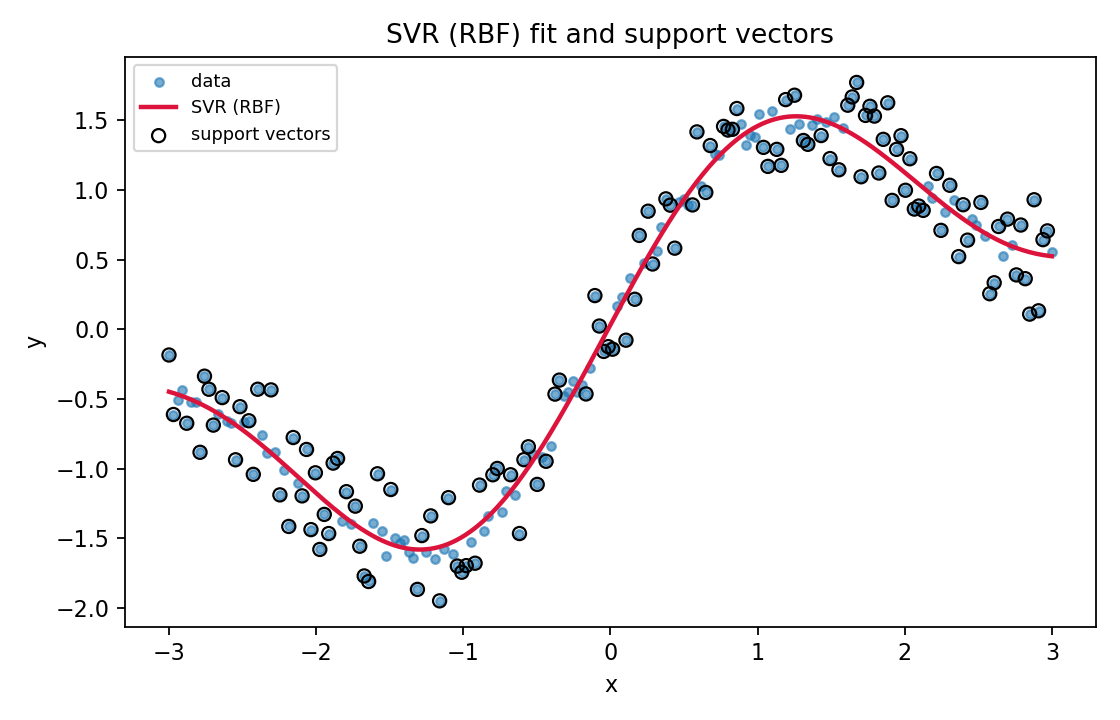
\includegraphics[width=0.85\linewidth]{svr_rbf_fit.png}
  \caption{SVR (RBF) 拟合与支持向量(合成数据)}
  \label{fig:svr_rbf_fit}
\end{figure}

\begin{figure}[H]
  \centering
  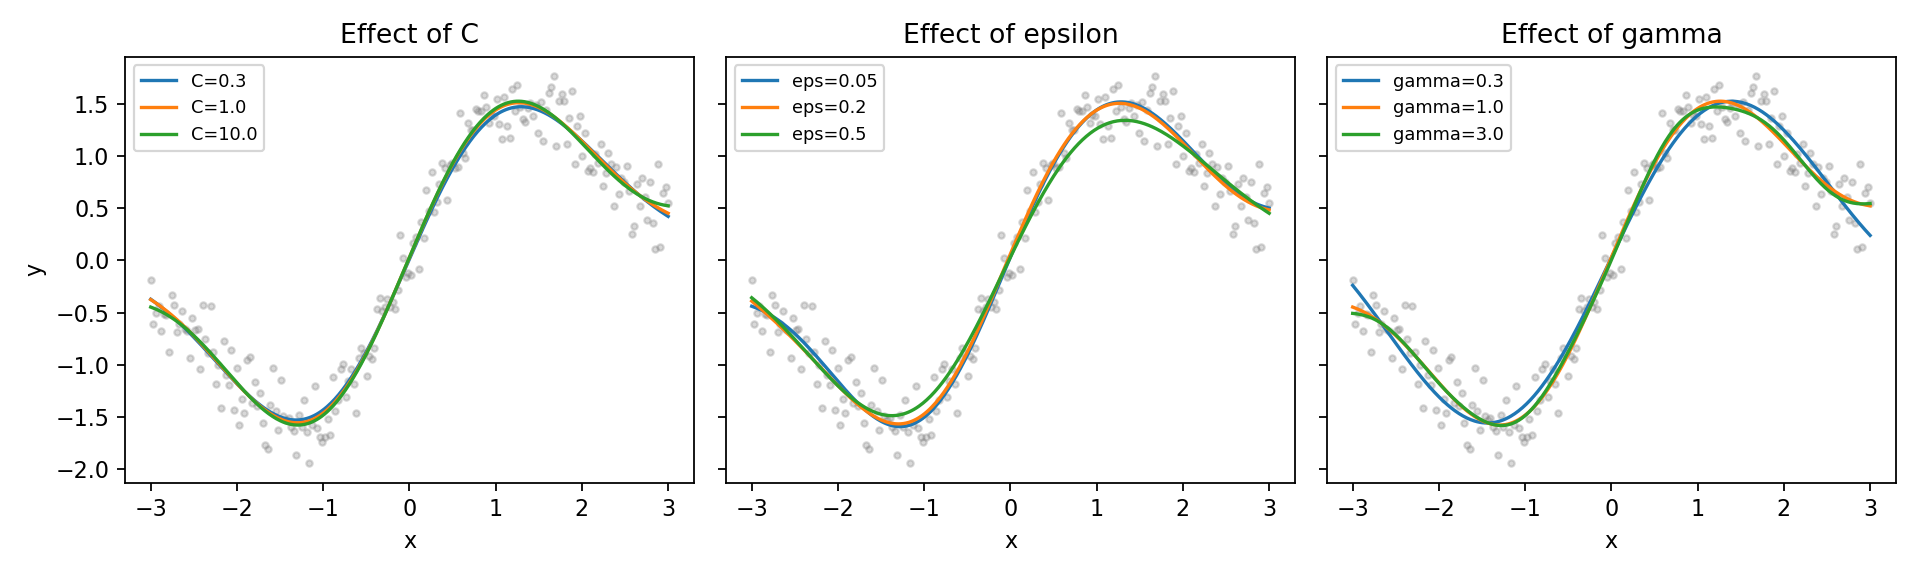
\includegraphics[width=0.95\linewidth]{svr_params_effect.png}
  \caption{超参数影响:改变 \(C\)、\(\varepsilon\)、\(\gamma\)}
  \label{fig:svr_params}
\end{figure}

\FloatBarrier % 阻止上面的图漂移到后续章节

\section{小结}
SVR 将大间隔与 \(\varepsilon\)-不敏感损失结合,并借助核函数处理非线性回归。实践中应标准化特征,并用交叉验证在对数尺度调参 \(C,\varepsilon,\gamma\),以获得稳健表现。

\end{document}

